%!TEX TS-program = xelatex
%----------------------------------------------------------------------------------------
%	PACKAGES AND THEMES
%----------------------------------------------------------------------------------------
\documentclass[aspectratio=169,xcolor=dvipsnames, t]{beamer}
\usepackage{fontspec}
\usepackage{unicode-math}
\setmathfont{latinmodern-math.otf}
\usepackage{hyperref}
\usepackage{graphicx}
\usepackage{booktabs}
\usepackage{tikz}
\usepackage{makecell}
\usepackage{wrapfig}
\usepackage[spanish]{babel}
\usepackage[numbers]{natbib}
\usepackage{subcaption}

% Tema personalizado
\usetheme{SimplePlusAIC}

%----------------------------------------------------------------------------------------
%	TITLE PAGE CONFIGURATION
%----------------------------------------------------------------------------------------

\title[Pronóstico de Violencia Extrema]{Fortalecimiento del SAT mediante Machine Learning en la detección de violencia atípica}
\subtitle{Seminario de Tesis}

\author[Heredia Niño]{Juan Diego Heredia Niño}
\institute[Universidad de los Andes]{Facultad de Economía \newline Universidad de los Andes}

\date{\today} 

%----------------------------------------------------------------------------------------
%	PRESENTATION SLIDES
%----------------------------------------------------------------------------------------

\begin{document}

\maketitlepage

\begin{frame}[t]{Contenido}
    \tableofcontents
\end{frame}

% En el archivo "sections/motivacion.tex"
\section{Motivación}

% Diapositiva 1: Costos de la Violencia
\begin{frame}{Los Costos de la Violencia}
    \begin{itemize}
        \item \textbf{Contexto en Latinoamérica:} 
        \begin{itemize}
            \item Hasta \alert{7.1\% del PIB} cuando se incluyen efectos intangibles (Londoño \& Guerrero, 1999).
        \end{itemize}
        
        \vspace{0.1cm}
        \pause
        \item \textbf{Contexto en Colombia:}
        \begin{itemize}
        \pause
            \item Costos \textbf{directos} superan \alert{3\% del PIB anual} (BID, 2017):
            \begin{itemize}
                \scriptsize
                \item Gasto público en seguridad/justicia
                \item Costo de victimización (homicidios)
                \item Inversiones privadas en protección
                \item Encarcelamiento
            \end{itemize}
        \pause
            \item Costos \textbf{indirectos}: %(difíciles de cuantificar)
            \begin{itemize}
                \item \alert{Productividad}: Pérdidas laborales y costos operativos empresariales
                \item \alert{Capital humano}: Reducción en inversión educativa y salud
                \item \alert{Instituciones}: Deterioro de confianza ciudadana
                \item \alert{Inversión}: Menor atracción de IED y planes de expansión
            \end{itemize}
        \end{itemize}
        
        
    \end{itemize}
\end{frame}
% Diapositiva 2: Impacto en el bienestar y violencia atípica
\begin{frame}{Impacto de la Violencia en el Bienestar}
    \begin{itemize}
        \item \textbf{Erosión multidimensional del bienestar}:
        \begin{itemize}
            \pause
            \item \alert{Finanzas públicas}: 
            \begin{itemize}
                \scriptsize
                \item Reducción de ingresos fiscales (salida de empresas + daño a infraestructura)
                \item Círculo vicioso: inseguridad $\rightarrow$ estancamiento $\rightarrow$ menos bienes públicos
            \end{itemize}
            \pause
            \item \alert{Capital humano:}
            \begin{itemize}
                \scriptsize
                \item Correlación negativa entre criminalidad y resultados educativos
                \item $\uparrow$ Brechas de desigualdad ($\downarrow$ movilidad social )
            \end{itemize}
            \pause
            \item \alert{Cohesión social}: Pérdida de confianza institucional + tejido social fracturado
        \end{itemize}
        
        \vspace{0.1cm}
        \pause
        \item \textbf{Violencia atípica:}
        \begin{itemize}
            \pause
            \item Episodios \alert{abruptos} e \alert{intensos}
            \item Menor capacidad de respuesta institucional
            \item Consecuencias críticas:
            \begin{itemize}
                \scriptsize
                \item Desplazamiento forzado + Pérdida de vidas
                \item Alteración organización socioeconómica/política
                \item Trauma colectivo
            \end{itemize}
        \end{itemize}
    \end{itemize}

\end{frame}


\begin{frame}{Sistema de Alertas Tempranas}
    \begin{itemize}
        % --- Primer clic: Definición y objetivo ---
        \item \textbf{¿Qué es el Sistema de Alertas Tempranas (SAT)?}
        \begin{itemize}
            \item Creado por la Defensoría del Pueblo en 2001
            \item Mecanismo institucional para \alert{monitorear riesgos} del conflicto armado
            \item Objetivo: Prevenir violaciones masivas de DDHH y proteger comunidades vulnerables
        \end{itemize}
        \pause
        
        % --- Segundo clic: Funcionamiento ---
        \vspace{0.3cm}
        \item \textbf{¿Cómo opera?}
        \begin{itemize}
    
            \item Metodología \alert{cualitativa}:
            \begin{itemize}
            
                \item Recopilación de testimonios, indicadores sociales y observación de campo
                \item Verificación humana de fuentes locales
            \end{itemize}
            \item Productos clave:
            \begin{itemize}
            
                \item Informes de Riesgo + Notas de Seguimiento
                \item Coordinación con entidades estatales para acción preventiva
            \end{itemize}
        \end{itemize}
    \end{itemize}
    

\end{frame}
\begin{frame}{Sistema de Alertas Tempranas}
    \begin{itemize}
        % --- Primer clic: Logros y desafíos ---
        \item \textbf{Logros y limitaciones:}
        \begin{itemize}
            
            \item \alert{Cobertura nacional}: 22 departamentos monitoreados (urbano + rural)
            \item \alert{Desafíos operativos}:
            \begin{itemize}
                
                \item Escalabilidad limitada por métodos manuales
                \item Detección tardía de señales no lineales (ej: violencia atípica)
                \item Dependencia de articulación interinstitucional
            \end{itemize}
        \end{itemize}
        \pause
        
        % --- Segundo clic: Oportunidad ML ---
        \vspace{0.1cm}
        \item \textbf{\alert{Complementar}} metodologías cualitativas
        \begin{itemize}
            \item Detección temprana de patrones en datos cuantitativos
            \item Priorización automática de zonas críticas
            \item Reducción de sesgos en interpretación humana
        \end{itemize}
    \end{itemize}

\end{frame}
\begin{frame}{¿Cómo se puede complementar el SAT usando Machine Learning?}
    \begin{itemize}
        % --- Parte 1: Por qué ML en violencia atípica ---
        \item \textbf{Violencia atípica: un desafío para métodos tradicionales}
        \begin{itemize}
            \item Factores detonantes: \alert{cambios abruptos} + variables no observables (ej: tensiones políticas locales)
            \item Dificultad para detectar relaciones \alert{no lineales} entre variables
            \item \alert{ML como solución}: Procesa múltiples fuentes + identifica patrones históricos complejos
        \end{itemize}
        \pause
        
        % --- Parte 2: Evidencia desde la literatura ---
        \vspace{0.1cm}
        \item \textbf{Lecciones de estudios recientes: Bazzi et al. (2022)}
        \begin{itemize}
            \item Análisis en Colombia e Indonesia con modelos predictivos:
            \begin{itemize}
                \item \alert{Acierto}: Identificación precisa de hotspots de violencia crónica
                \item \alert{Falla}: Baja precisión en predicción de brotes nuevos
            \end{itemize}
            \item Implicación clave: Combinar \alert{ML} con \alert{análisis cualitativo} del SAT
        \end{itemize}

    \end{itemize}
\end{frame}
\begin{frame}{Determinantes de la Violencia en Colombia}
    \begin{itemize}
        \item \textbf{¿Por qué estudiar los determinantes?}
        \begin{itemize}
            \item Entender las causas subyacentes es clave para:
            \begin{itemize}
                \item Diseñar modelos predictivos robustos (ej: ML + SAT)
                \item Priorizar variables en análisis de riesgo
                \item Evitar soluciones simplistas o descontextualizadas
            \end{itemize}
        \end{itemize}
        
        \vspace{0.4cm}
        
        \item \textbf{Enfoque integrado: Levitt \& Rubio (2000); Bourguignon et al. (2003)}
        \begin{itemize}
            \item \alert{Factores estructurales} (largo plazo):
            \begin{itemize}
                \item Desigualdad, debilidad institucional, economías ilegales
            \end{itemize}
            
            \item \alert{Incentivos económicos} (corto plazo):
            \begin{itemize}
                \item Rentas ilícitas, control de recursos, alta impunidad
            \end{itemize}
        \end{itemize}
    \end{itemize}

\end{frame}
\begin{frame}{Determinantes de la Violencia en Colombia}
    \begin{itemize}
        \item \textbf{Factores estructurales críticos}:
        \begin{itemize}
            \item \alert{Debilidad institucional}: 
            \begin{itemize}
                \item Bonilla (2009): 75\% de homicidios no resueltos en zonas rurales 
            \end{itemize}
            
            \item \alert{Desigualdad socioeconómica}:
            \begin{itemize}
                \item Bourguignon et al. (2003): +1\% desempleo juvenil $\rightarrow$ +0.8\% homicidios
            \end{itemize}
        \end{itemize}
        
        \vspace{0.4cm}
        
        \item \textbf{Incentivos económicos y choques externos}:
        \begin{itemize}
            \item \alert{Bonanzas de commodities}:
            \begin{itemize}
                \item Dube \& Vargas (2013): +10\% precio petróleo $\rightarrow$ +6.5\% violencia
            \end{itemize}
            
            \item \alert{Narcotráfico}:
            \begin{itemize}
                \item Angrist \& Kugler (2008): Regiones con coca tienen 3x más masacres
            \end{itemize}
        \end{itemize}
    \end{itemize}

\end{frame}
\begin{frame}{Enfoque Analítico del Estudio}
    \vspace{0.4cm}
\textbf{Perspectiva de violencia:} \alert{Seguridad pública}
        \pause
        \vspace{0.2cm}
        \begin{itemize}
            \item Incidencia de \alert{grupos armados} y \alert{criminales}:
            \begin{itemize}
                \item Economías ilícitas
                \item Control territorial
                \item Confrontación armada
            \end{itemize}
            
            \vspace{0.4cm}
            \pause
            \item Impacto de la violencia: 
            \begin{itemize}
                \item Vida cotidiana de la población
                \item Gobernanza local 
                \item Estabilidad institucional
            \end{itemize}
        \end{itemize}

\end{frame}
% En el archivo "sections/hechos_estilizados.tex"
\section{Hechos Estilizados}

\begin{frame}{Presencia de Grupos Armados}
    \begin{figure}[ht]
        \centering
        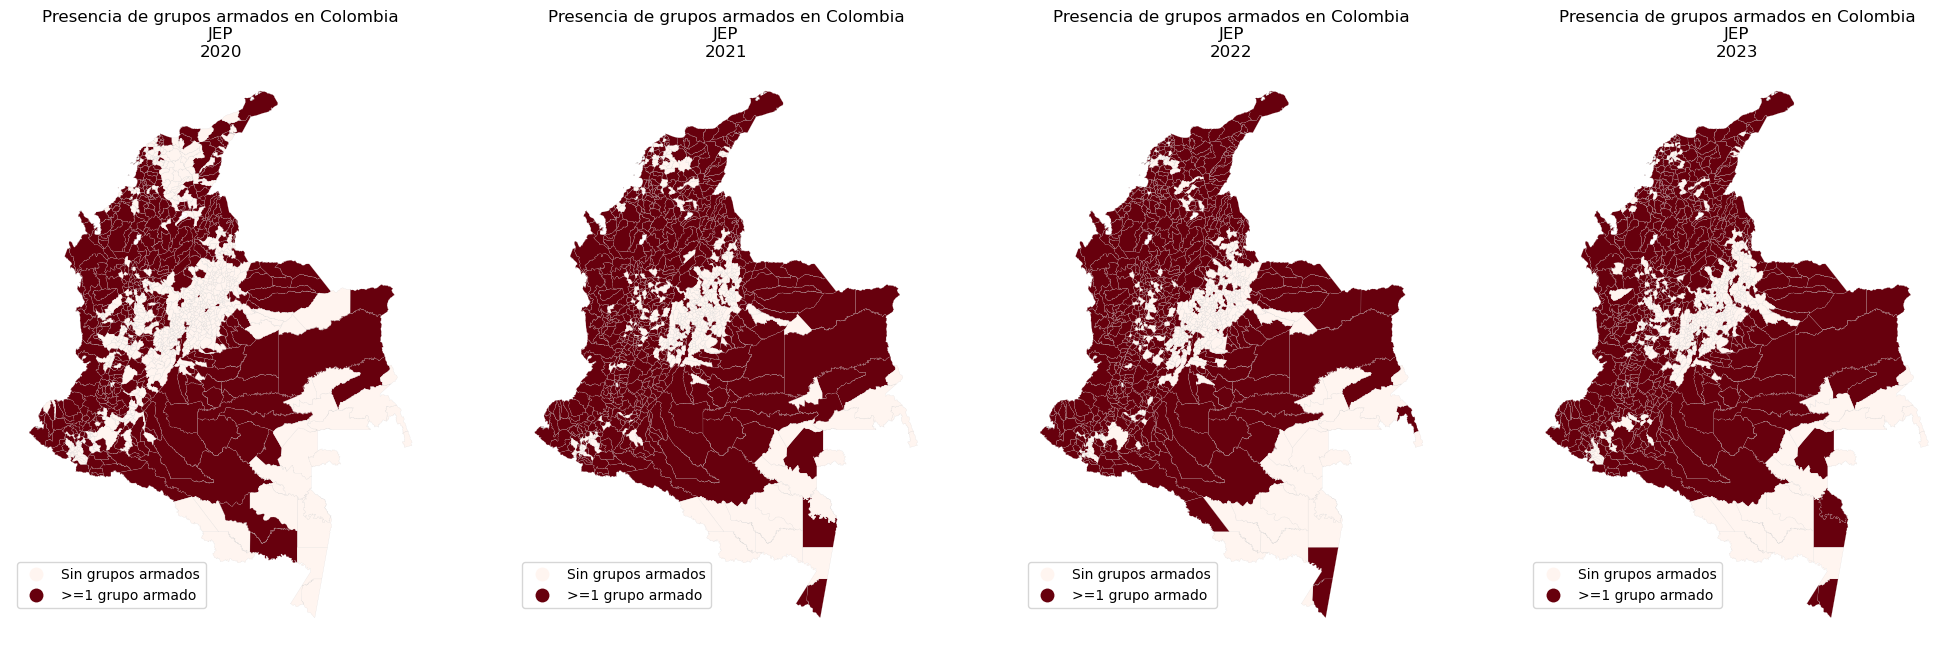
\includegraphics[width=1\textwidth, height=0.6\textheight, keepaspectratio]{images/image.png}
        \caption{\footnotesize Expansión de grupos armados por municipios en Colombia, 2020-2023}
    \end{figure}

    \centering
    \footnotesize\textit{Fuente: Elaboración propia}
\end{frame}

\begin{frame}{Presencia de Grupos Criminales}
    \begin{figure}[ht]
        \centering
        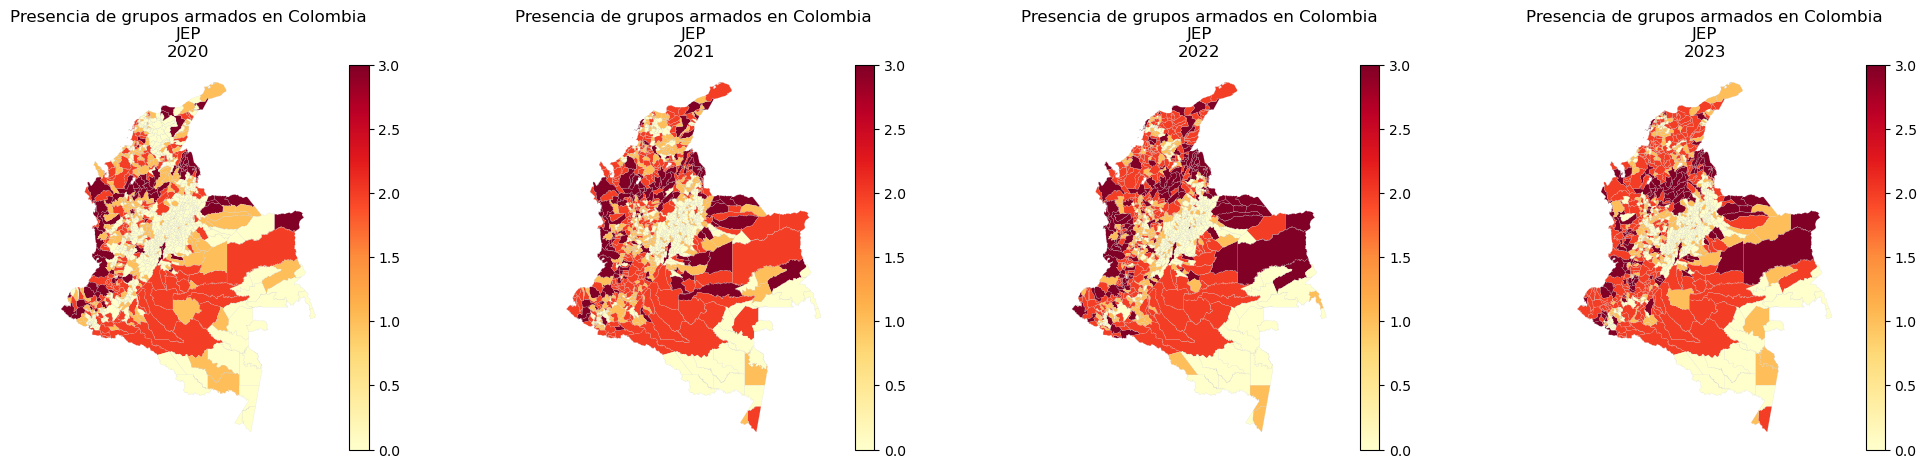
\includegraphics[width=1\textwidth, height=0.6\textheight, keepaspectratio]{images/image 1.png}
        \caption{\footnotesize Cantidad de grupos armados por municipios en Colombia, 2020-2023}
    \end{figure}

    \centering
    \footnotesize\textit{Fuente: Elaboración propia}
\end{frame}


\begin{frame}{¿Qué definimos por violencia?}
    \pause
    \begin{block}{Índice de Violencia Agregada (IACV)}
        \begin{itemize}
            \item Componentes (Municipal y trimestral por 100,000 hab.):
            \begin{itemize}
                \item Homicidio, extorsión, secuestro, terrorismo, masacres
            \end{itemize}
            \item Ponderación por gravedad legal (Código Penal):
        \end{itemize}
        
        \centering
        \begin{tabular}{lcc}
            \toprule
            \textbf{Delito} & \textbf{Pena (años)} & \textbf{Peso (\%)} \\
            \midrule
            Homicidio & 19.0 & 17.04 \\
            Extorsión & 11.5 & 10.31 \\
            Secuestro & 16.0 & 14.35 \\
            Terrorismo & 15.0 & 13.45 \\
            Masacres & 50.0 & 44.84 \\
            \midrule
            
            \bottomrule
        \end{tabular}
        \begin{itemize}
        \item \alert{Propósito}: Medida de seguridad pública agregada
        \end{itemize}
    \end{block}

\end{frame}

\begin{frame}{¿Qué otros tipos de violencia definimos?}
    \pause
    \begin{columns}[T]
        \begin{column}{0.48\textwidth}
            \begin{block}{Índice de Amedrentamiento (IA)}
                \begin{itemize}
                    \item Componentes (Municipal y trimestral por 100,000 hab.):
                    \begin{itemize}
                        \item Amenazas
                        \item Tentativas de asesinato y atentados
                        \item Desplazamiento forzado
                        \item Hostigamiento
                    \end{itemize}
                    \item \alert{Propósito}: Medir clima de miedo
                \end{itemize}
            \end{block}
        \end{column}
        
        \begin{column}{0.48\textwidth}
            \begin{block}{Índice de Gobernanza Criminal (IGC)}
                \begin{itemize}
                    \item Componentes (Municipal y trimestral por 100,000 hab.):
                    \begin{itemize}
                        \item Confinamientos
                        \item Retenes ilegales
                        \item Paros armados
                        \item Extorsión
                    \end{itemize}
                    \item \alert{Propósito}: Medir control territorial
                \end{itemize}
            \end{block}
        \end{column}
    \end{columns}
\end{frame}

\begin{frame}{Evolución de la Violencia en Colombia}
    \begin{figure}[ht]
        \centering
        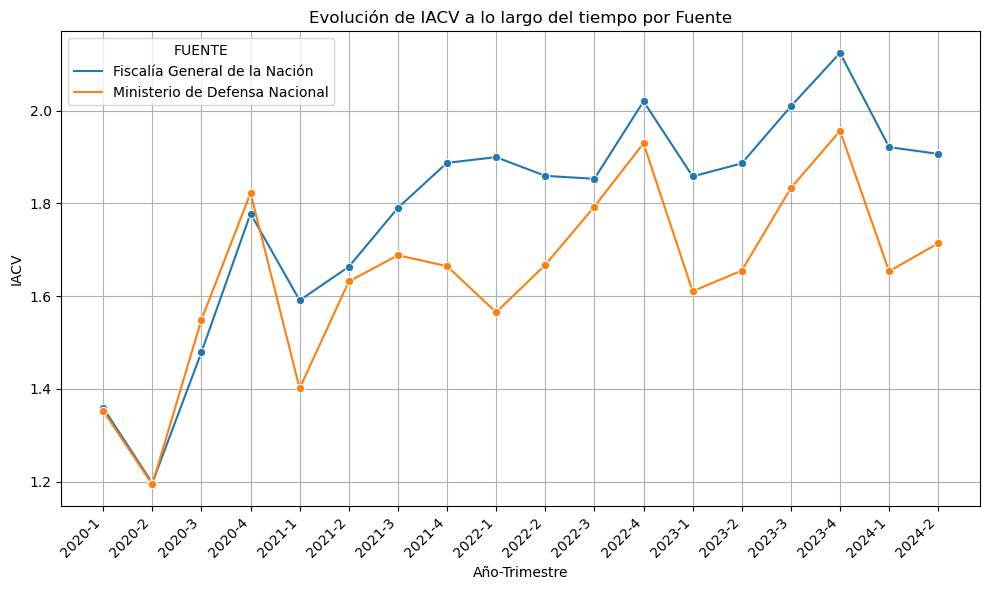
\includegraphics[width=0.9\textwidth, height=0.7\textheight, keepaspectratio]{images/image 7.png}
    \end{figure}
    \centering
    \footnotesize\textit{Fuente: Elaboración propia}
\end{frame}

\begin{frame}{Distribución de la violencia en Colombia}
    \begin{columns}[T]
        % Columna izquierda
        \begin{column}{0.48\textwidth}
            \centering
            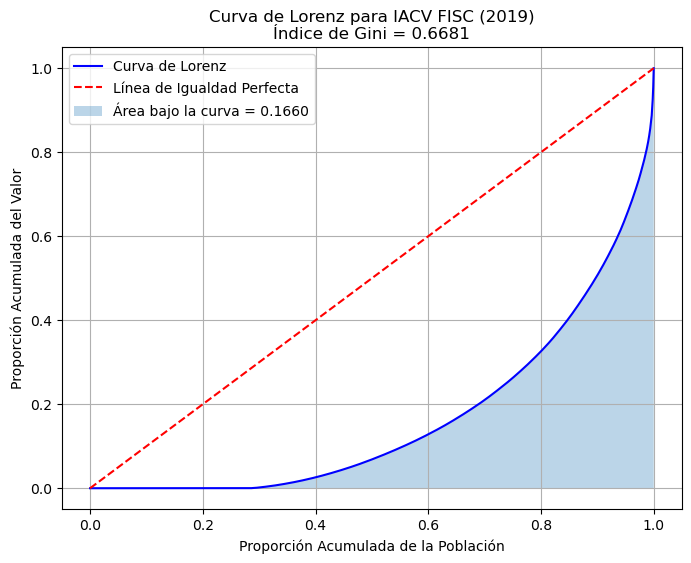
\includegraphics[width=\textwidth, height=0.65\textheight, keepaspectratio]{images/image 3.png}
        \end{column}
        
        % Columna derecha
        \begin{column}{0.48\textwidth}
            \centering
            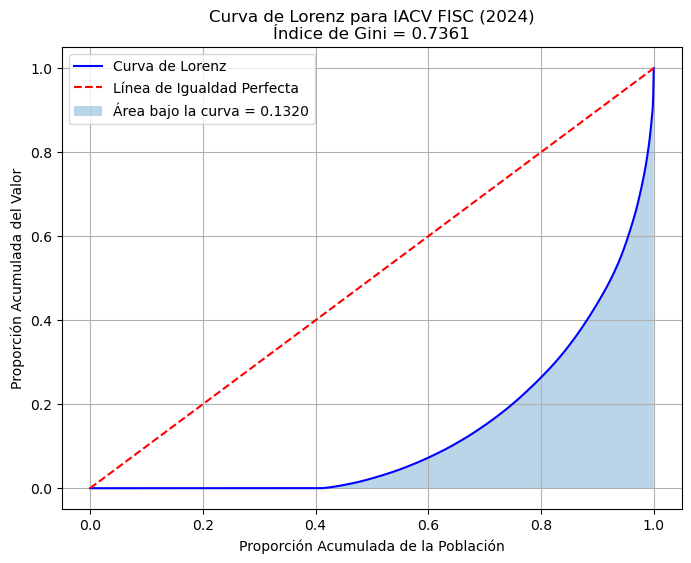
\includegraphics[width=\textwidth, height=0.65\textheight, keepaspectratio]{images/image 4.png}
        \end{column}
    \end{columns}
    \vspace{0.2cm}
    \centering
    \footnotesize\textit{Fuente: Elaboración propia}
\end{frame}


\begin{frame}{Vulnerabilidad municipal a la violencia}
    \begin{columns}[T]
        % Columna izquierda
        \begin{column}{0.48\textwidth}
            \centering
            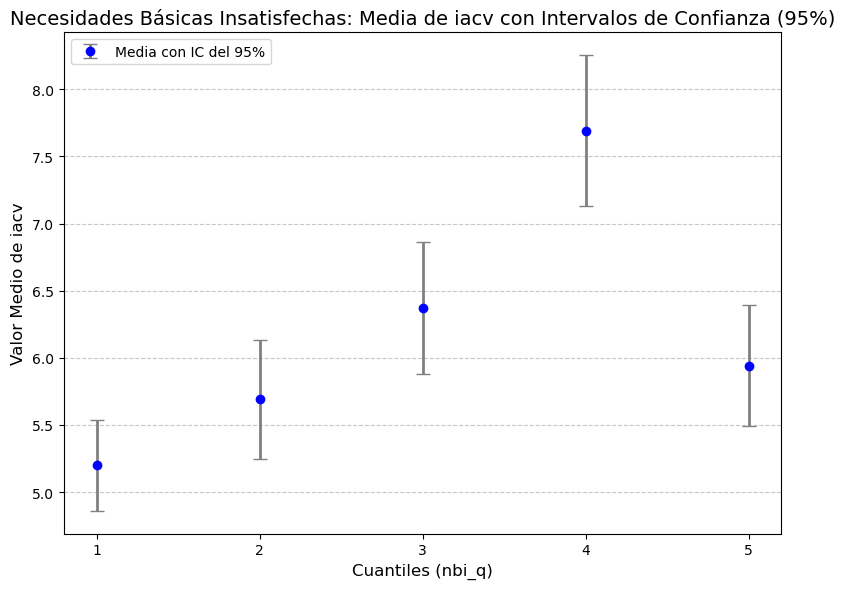
\includegraphics[width=\textwidth, height=0.65\textheight, keepaspectratio]{images/output1.png}
        \end{column}
        
        % Columna derecha
        \begin{column}{0.48\textwidth}
            \centering
            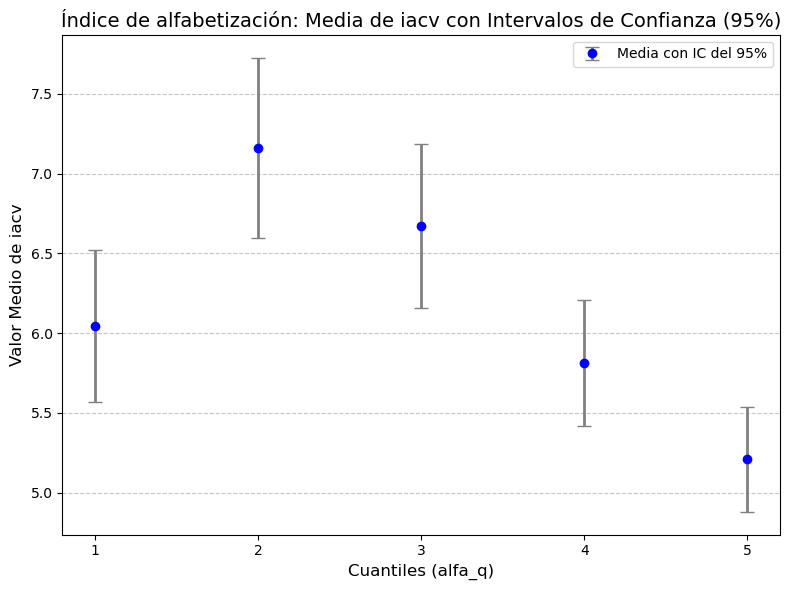
\includegraphics[width=\textwidth, height=0.65\textheight, keepaspectratio]{images/output2.png}
        \end{column}
    \end{columns}
    \vspace{0.2cm}
    \centering
    \footnotesize\textit{Fuente: Elaboración propia}
\end{frame}

\makesection{Pregunta de Investigación}

\begin{frame}{}
    \vspace{3cm}
    \centering
    \Large ¿El uso de Machine Learning para pronosticar \hyperlink{violenciaatipica}{\alert{violencia atípica}} mejorará la
    \alert{precisión y sensibilidad} del pronóstico en comparación con las alertas tempranas de la Defensoría? 

\end{frame}

\begin{frame}{¿Qué entendemos por Violencia Atípica?}
     Criterio basado en \alert{desviación estándar}: Bazzi et al.(2022):
        \begin{block}{Definición}
        La \textbf{violencia atípica} se define como aquella que supera el umbral de 
        \textbf{1 desviación estándar} del promedio de los últimos \textbf{3 años}.
    \end{block}
\end{frame}

\begin{frame}{Problema de Clasificación Binaria}
    \begin{itemize}
        \item \textbf{Decisión operativa}: Atípico (1) vs No atípico (0)
        \begin{itemize}
            \item Más eficiente que predicción continua para el SAT
        \end{itemize}
        
        \item \alert{Ventajas clave}:
        \begin{itemize}
            \item Manejo de desbalance:
            \begin{itemize}
                \item Reponderación de clases
                \item Sobremuestreo controlado
            \end{itemize}
            
            \item Optimización de umbrales: Ajuste para maximizar F1-Score
        \end{itemize}
        
    \end{itemize}
\end{frame}

\begin{frame}{Métricas}
    \begin{columns}[T]
        % Columna izquierda (texto)
        \begin{column}{0.6\textwidth}
            \begin{itemize}
            \pause
                \item \textbf{Precisión}:
                \begin{itemize}
                    \item "No mover recursos innecesariamente"
                    \item Minimiza la cantidad de veces que pronostíco violencia atípica y no ocurre
                    \item \alert{Costo de fallar}: Desgaste institucional + gasto inútil
                \end{itemize}
                \pause
                \item \textbf{Sensibilidad}:
                \begin{itemize}
                    \item "No dejar pasar ningún evento crítico"
                    \item Minimiza la cantidad de veces que no pronostíco violencia atípica y ocurre
                    \item \alert{Costo de fallar}: Pérdida de vidas + crisis humanitaria
                \end{itemize}
                \pause
                \item \textbf{F1-Score}:
                \begin{itemize}
                    \item Balance entre eficiencia y protección
                \end{itemize}
            \end{itemize}
        \end{column}
        \pause
        % Columna derecha (ecuaciones)
        \begin{column}{0.4\textwidth}
            \centering

            \textbf{Precisión}
            \begin{align*}
                P = \frac{\text{VP}}{\text{VP} + \text{FP}}
            \end{align*}

            
            \textbf{Sensibilidad}
            \begin{align*}
                S = \frac{\text{VP}}{\text{VP} + \text{FN}}
            \end{align*}

            
            \textbf{F1-Score}
            \begin{align*}
                F1 = 2 \times \frac{P \times S}{P + S}
            \end{align*}
        \end{column}
    \end{columns}
\end{frame}

\makesection{Datos}
\begin{frame}{Fuentes de Datos}
Los datos de violencia provienen de tres fuentes principales:

\begin{itemize}
    \item \textbf{Fiscalía General de la Nación}: Registros mensuales de \alert{homicidio, extorsión, secuestro, terrorismo y masacres} a nivel municipal, mensual (2014-2024).
    \item \textbf{Ministerio de Defensa Nacional}: Serie histórica de los mismos delitos con \alert{mayor cobertura temporal} a nivel municipal, mensual(1997-2024)%, permitiendo análisis de tendencias a largo plazo. Idea para hacer PCA para los datos antes del corte de la fiscalía
    \item \textbf{Jurisdicción Especial para la Paz (JEP)}: Datos sobre \alert{presencia de grupos armados y eventos violentos} (2017-2024), incluyendo desplazamientos, hostigamientos y paros armados.
\end{itemize}
\end{frame}
\begin{frame}{Fuentes de Datos}

Para analizar la relación entre violencia y factores estructurales, se integran:

\begin{itemize}
    \item \textbf{Panel Municipal del CEDE} (2005-2023): Información demográfica, socioeconómica e institucional, como \alert{pobreza, acceso a servicios y programas para víctimas}.
    \item \textbf{Cultivos ilícitos de coca} (1999-2023, Observatorio de Drogas de Colombia): Financiación de grupos armados y la \alert{dinámica del conflicto}.
    \item \textbf{Luminosidad nocturna (VIIRS Nighttime Light)} (2012-2023): Indicador proxy de \alert{actividad económica local}.
\end{itemize}
\end{frame}

\makesection{Metodología}

\begin{frame}{Modelo Teórico: Clasificación Binaria}

    \begin{itemize}
        \item \alert{Aprendizaje Supervisado}: \textbf{Clasificación Binaria}
        $$y = f(X)$$
        \pause
        \item \textbf{Función de probabilidad}:
        \[
        y_t = \begin{cases} 
            1 & \text{si } \text{IACV}_t \geq \bar{X} + \sigma \text{ (atípico)} \\
            0 & \text{si } \text{IACV}_t < \bar{X} + \sigma \text{ (normal)}
        \end{cases}
        \]
        \end{itemize}
\end{frame}





\begin{frame}{Estimación}
    \begin{alertblock}{Objetivo}
        Estimar \( P(y=1|X) \) para activar alertas tempranas con \( \uparrow \) precisión y \( \uparrow \) sensibilidad
    \end{alertblock}
    \pause
    \begin{itemize}
        \item \textbf{Variables explicativas \( X \)}:
        \pause
        \begin{itemize}
            \item \alert{Factores estructurales}:
            \begin{itemize}
                \footnotesize
                \item Desigualdad, presencia estatal, economías ilegales, empleo, presencia grupos armados, educación, ubicación, etc.
            \end{itemize}
            \pause
            \item \alert{Rezagos temporales de violencia}:
            \begin{itemize}
                \footnotesize
                \item IACV, IGC e IA
            \end{itemize}
        
        \end{itemize}
        \end{itemize}
\end{frame}




\begin{frame}{Enfoques de Machine Learning: Elastic Net y Random Forest}
    \begin{columns}[T]
        \begin{column}{0.48\textwidth}
            \begin{alertblock}{1. Elastic Net}
                \begin{itemize}
                    
                    \item \textbf{Qué hace}: 
                    \begin{itemize}
                        
                        \item Regresión lineal con penalización combinada L1 (Lasso) y L2 (Ridge)
                    \end{itemize}
                    \item \textbf{Ventaja}: 
                    \begin{itemize}
                        
                        \item Selección automática de variables y reducción de sobreajuste
                    \end{itemize}
                \end{itemize}
            \end{alertblock}
        \end{column}
        
        \begin{column}{0.48\textwidth}
            \begin{alertblock}{2. Random Forest}
                \begin{itemize}
                    
                    \item \textbf{Qué hace}: 
                    \begin{itemize}
                        
                        \item Ensamble de múltiples árboles de decisión
                    \end{itemize}
                    \item \textbf{Ventaja}: 
                    \begin{itemize}
                        
                        \item Maneja alta dimensionalidad y reduce el sobreajuste
                    \end{itemize}
                \end{itemize}
            \end{alertblock}
        \end{column}
    \end{columns}
\end{frame}

\begin{frame}{Enfoques de Machine Learning: XGBoost y LSTM}
    \begin{columns}[T]
        \begin{column}{0.48\textwidth}
            \begin{alertblock}{3. XGBoost}
                \begin{itemize}
                    
                    \item \textbf{Qué hace}: 
                    \begin{itemize}
                        
                        \item Boosting con n iteraciones + regularización
                    \end{itemize}
                    \item \textbf{Ventaja}: 
                    \begin{itemize}
                        \item Similar a Random Forest
                        \item Eficiencia con datos desbalanceados
                        \item Tratamiento de valores nulos
                    \end{itemize}
                \end{itemize}
            \end{alertblock}
        \end{column}
        
        \begin{column}{0.48\textwidth}
            \begin{alertblock}{4. Redes LSTM}
                \begin{itemize}
                    
                    \item \textbf{Qué hace}: 
                    \begin{itemize}
                        
                        \item Modela dinámicas temporales de forma más efectiva que métodos tradicionales
                    \end{itemize}
                    \item \textbf{Ventaja}: 
                    \begin{itemize}
                        
                        \item Detecta patrones temporales críticos 
                    \end{itemize}
                \end{itemize}
            \end{alertblock}
        \end{column}
    \end{columns}

\end{frame}
\begin{table}[H]
\centering
\begin{tabular}{lrrrr}
\toprule
 & \textbf{Logit} & \textbf{Lasso} & \textbf{Elastic Net} & \textbf{Random Forests} \\
\midrule
AUC             & 0.811302 & 0.811277 & 0.811276 & 0.897908 \\
Sensibilidad    & 0.743353 & 0.743425 & 0.743425 & 0.603754 \\
Especificidad   & 0.707203 & 0.707058 & 0.707038 & 0.996758 \\
\% Acierto      & 0.720374 & 0.720309 & 0.720296 & 0.853565 \\
Relación FP/TP  & 0.687167 & 0.687439 & 0.687488 & 0.009368 \\
Relación FN/TP  & 0.345255 & 0.345125 & 0.345125 & 0.656304 \\
\bottomrule
\end{tabular}
\caption{Comparación de modelos: métricas de desempeño}
\label{tab:model_comparison}
\end{table}


\begin{frame}{}
    \vspace{3.5cm}
    \centering
    \LARGE \alert{\textbf{¡Gracias!}} 

\end{frame}

\begin{frame}{Referencias}

\begin{itemize}
\tiny
    \item Banco Interamericano de Desarrollo. (2017). \textit{Los costos del crimen y la violencia}. Banco Interamericano de Desarrollo. \url{https://doi.org/10.18235/0006383}

    \item Bazzi, S., Blair, R. A., Dube, O., Gudgeon, M., \& Peck, R. (2022). \textit{The promise and pitfalls of conflict prediction: Evidence from Colombia and Indonesia}. \textit{The Review of Economics and Statistics, 104}(6), 1246–1262. \url{https://doi.org/10.1162/rest_a_01172}
    
    \item Bourguignon, F., Núñez, J., \& Sánchez, F. (2003). \textit{What part of the income distribution does inequality affect crime? The case of Colombia}. Documento CEDE, Universidad de los Andes.

    \item Dube, O., \& Vargas, J. F. (2013). \textit{Commodity price shocks and civil conflict: Evidence from Colombia}. \textit{Review of Economic Studies, 80}(4), 1384–1421. \url{https://doi.org/10.1093/restud/rdt009}

    \item Feldmann, A., \& Hinojosa, V. (2009). \textit{Terrorism in Colombia: Logic and sources of a multidimensional and ubiquitous phenomenon}. \textit{Terrorism and Political Violence, 21}(1), 42-61. \url{https://doi.org/10.1080/09546550802544694}

    \item Levitt, S., \& Rubio, M. (2000). \textit{Understanding crime in Colombia and what can be done about it}. Documento de trabajo, Universidad de Chicago/Fedesarrollo.

    \item Londoño, J. L., \& Guerrero, R. (1999). \textit{Violencia en América Latina: Epidemiología y costos}. Banco Interamericano de Desarrollo.

    \item Mejía, D., \& Restrepo, P. (2011). \textit{The economics of the war on illegal drug production and trafficking}. Documento CEDE, Universidad de los Andes.

    \item Rubio, M. (2003). \textit{El rapto de la pesca milagrosa: Breve historia del secuestro en Colombia}. Documentos CEDE No. 2003-36, Universidad de los Andes.

    \item Sánchez, F., \& Chacón, M. (2005). \textit{Conflicto, Estado y descentralización: Disputa armada por el control local, 1974–2002}. Documento CIDER/Universidad de los Andes – LSE.


\end{itemize}
\end{frame}

\end{document}

